%
\documentclass{acmtog}
\usepackage{indentfirst}
\usepackage[utf8]{inputenc}
\usepackage{amsmath}
\usepackage[retainorgcmds]{IEEEtrantools} %IEEEeqnarray
\usepackage{listings}
\usepackage{hyperref}

\lstset{
    language=C,
    tabsize=2,
    breakatwhitespace=false,
    basicstyle=\ttfamily\footnotesize\bfseries,
    captionpos=b,
}

\renewcommand*{\lstlistingname}{Listing}

\acmVolume{VV}
\acmNumber{N}
\acmYear{YYYY}
\acmMonth{Month}
\acmArticleNum{XXX}  
\acmdoi{10.1145/XXXXXXX.YYYYYYY}

\acmVolume{}
\acmNumber{}
\acmYear{2012}
\acmMonth{02}
\acmArticleNum{}
\acmdoi{}

\begin{document}

\markboth{Miguel Palhas}{Overview of Lindenmayer Systems}

\title{Overview of Lindenmayer Systems} % title

\author{Miguel Palhas
\affil{Universidade do Minho}}

%\category{I.3.7}{Computer Graphics}{Three-Dimensional Graphics and Realism}[Animation]
%\category{I.3.5}{Computer Graphics}{Computational Geometry and Object Modeling}[Physically based modeling]

%\terms{Experimentation, Human Factors}

%\keywords{Face animation, image-based modelling, iris animation, photorealism, physiologically-based modelling}

%\acmformat{Pamplona, V. F., Oliveira, M. M., and Baranoski, G. V. G. 2009. Photorealistic models for pupil light
%reflex and iridal pattern deformation.  {ACM Trans. Graph.} 28, 4, Article 106 (August 2009), 11 pages.\newline  DOI $=$
%10.1145/1559755.1559763\newline http://doi.acm.org/10.1145/1559755.1559763}

\maketitle

%\begin{bottomstuff} 
%Manuel M. Oliveira acknowledges a CNPq-Brazil fellowship (305613/2007-3). Gladimir V. G. Baranoski acknowledges a
%NSERC-Canada grant (238337). Microsoft Brazil provided additional support.
%
%Authors' addresses: land and/or email addresses.
%\end{bottomstuff}

\begin{abstract}
[Abstact here]
 % We introduce a physiologically-based model for pupil light reflex (PLR) and an image-based model for iridal pattern
%deformation. Our PLR model expresses the pupil diameter as a function of the lighting of the  environment, and is
%described by a delay-differential equation, naturally adapting the pupil diameter even to abrupt changes in light
%conditions. Since the parameters of our PLR model were derived from measured data, it correctly simulates the actual
%behavior of the human pupil. Another contribution of our work is a model for realistic deformation of the iris pattern as a
%function of pupil dilation and constriction. Our models produce high-fidelity appearance effects and can be used to
%produce real-time predictive animations of the pupil and iris under variable lighting conditions. We assess the
%predictability and quality of our simulations  through comparisons of modeled results against measured data derived from
%experiments also described in this work. Combined, our models can bring facial animation to new photorealistic
%standards. Another contribution of our work is a model for realistic deformation of the iris pattern as a
%function of pupil dilation and constriction. Another contribution of our work is a model for realistic deformation of the iris pattern as a
%function of pupil dilation and constriction.  Another contribution of our work is a model for realistic deformation of the iris pattern as a
%function of pupil dilation and constriction.
\end{abstract}


%%%%%%%%%%%%%%%%%%%%%%%%%%%%%%%%%%%%%%%%%%%%%%%%
%%%%%%%%%%%%%%%%%%%%%%%%%%%%%%%%%%%%%%%%%%%%%%%%
\section{Origin}
\label{sec:origin}

L-Systems were introduced in 1968 by a Hungarian biologist, Aristid Lindenmayer. Lindenmayer studied the patterns that can be observed in the growth of several types of plants. The original idea was to provide a formal method of describing the development of simple organisms. Later on, they started to be used to for more complex structures.



%end sec{origin}

%%%%%%%%%%%%%%%%%%%%%%%%%%%%%%%%%%%%%%%%%%%%%%%%
%%%%%%%%%%%%%%%%%%%%%%%%%%%%%%%%%%%%%%%%%%%%%%%%
\section{Basic Structure and Properties}
\label{sec:basicstruct}

A Lindenmayer system (more commonly known simply as L-system) is a type of rewriting system, a general tool for constructing complex objects by starting with a simple object and recursively replacing parts according to instructions provided by a set of rewriting rules.

Formally, an L-System is a grammatical method to proceduraly model a system. It is generically represented as:

\begin{equation}
  G = (V, \omega , P)
  \label{eq:genericsystem}
\end{equation}

where:
\begin{description}
  \item[\textbf{V}] is the alphabet, a set of symbols defining the elements that compose the language of system we are describing. These symbols can be concatenated into strings;
  \item[\textbf{$\omega$}] is the axiom, or the initial string upon which the system will operate to generate the final geometry;
  \item[\textbf{P}] is the set of production rules, that define how the strings are replaced to form new combinations.
\end{description}

It's also necessary to provide a depth level ($n$), to indicate how deeply the productions should be processed, to control the level of detail of the final geometry.

These are the components of a regular grammar, from which L-Systems are derived. Aside from those attributes, the system must also define a translation mechanism which maps each of the resulting strings into a geometric structure, in order to generate the final result.

The system works by applying the rules iteratively to a string, whose initial value is given by w. As oposed to a conventional formal grammar, which applies a single rule at a time, in this case many rules can be applied simultaneously in a single iteration.

If each production refers only to an individual symbol and to its neighbours, the system is considered to be context-free. This subset of L-Systems are specified by a regular grammar. If the rules depend also on the neighbour symbols, then it is a context-sensitive L-System.

An L-System can also be non-deterministic or deterministic. If only one rule can apply to each symbol, then it is deterministic, as the final result will not change as long as neither of the initial parameters also remain the same. However, there may be several rules applying to the same symbols, and a defined method of selecting between each one. If this method is probabilistic, then the system is a stochastic L-System.

%end sec{basic structure and properties}

%%%%%%%%%%%%%%%%%%%%%%%%%%%%%%%%%%%%%%%%%%%%%%%%
%%%%%%%%%%%%%%%%%%%%%%%%%%%%%%%%%%%%%%%%%%%%%%%%
\section{Example}
\label{sec:example}

shows the original example showed by Lindenmayer, which models the growth of algae:
\begin{eqnarray}
  V   &=& \{A, B\}           \nonumber  \\
  \omega       &=& A                  \nonumber  \\
  P       &=& \{A \rightarrow AB,  \nonumber  \\
              & & B \rightarrow A \}  \nonumber
  \label{eq:example1}
\end{eqnarray}


this system produces the following result on the first iterations:

\begin{IEEEeqnarray}{l}
  n=0: A \nonumber \\
  n=1: AB \nonumber \\
  n=2: ABA \nonumber \\
  n=3: ABAAB \nonumber \\
  n=4: ABAABABA \nonumber
\end{IEEEeqnarray}

The recursive nature of the system can be seen in this example, as the resultant string becomes larger with every iteration

%%%%%%%%%%%%%%%%%%%%%%%%%%%%%%%%%%%%%%%%%%%%%%%%
%%%%%%%%%%%%%%%%%%%%%%%%%%%%%%%%%%%%%%%%%%%%%%%%
\section{Rendering}
\label{sec:rendering}

After defining the grammar for the desired model, a method is required to generate a graphical imagem based on the symbols acquired from iterating through the grammar. A common method to perform this is with Turtle graphics.

Turtle graphics is a computer graphics technique used for vector graphics that works a state machine using a cursor (also called the "turtle") in a Cartesian Plane. In this method, commands are given to alter the state of the turtle, which has simple properties like position, orientation, color, or drawing state. When the drawing state is true, the turtle acts like a pen, drawing as it moves. The turtle can receive commands such as "\textit{move forward 5 units}" or "\textit{turn left by 30 degrees}", effectively altering the current state.

From this basic building blocks, more complex algorithms can be made. Consider the following function that instructs the turtle to draw a simple square:

\begin{lstlisting}[label={lst:square}]
  draw_box() {
    forward(10);
    turn(90);
    forward(10);
    turn(90);
    forward(10);
    turn(90);
    forward(10);
    turn(90); 
  }
\end{lstlisting}

This function can then be used to draw even more complex shapes, such as a group of boxes:

\begin{lstlisting}[caption={},label={lst:squares}]
  draw_boxes() {
    draw_box();
    turn(90);
    draw_box();
    turn(90);
    draw_box();
    turn(90);
    draw_box();
    turn(90);
  }
\end{lstlisting}

\autoref{fig:boxes} illustrates the result of both this functions.

\begin{figure}[!htp]
  \begin{center}
    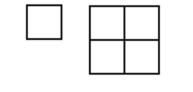
\includegraphics{images/0_draw_box}
    \caption{Squares drawn with turtle graphics \label{fig:boxes}}
    \end{center}
\end{figure}

Of course, the amount of instructions that can be issued to the turtle is implementation-dependant, and can be much more complex as just moving forward and rotating. Concepts like memory, stacks, probabilities and functions can be implemented to further increase the capabilities of the turtle.

%%%%%%%%%%%%%%%%%%%%%%%%%%%%%%%%%%%%%%%%%%%%%%%%
%%%%%%%%%%%%%%%%%%%%%%%%%%%%%%%%%%%%%%%%%%%%%%%%
\section{Pairing L-Systems with Turtle Graphics}
\label{sec:pairing}

In an L-System, strings are recursively expanded into other strings based on the set of production. If we interpret each Symbol of a string as a turtle command, then we can look at the whole string given by the L-System as a whole function that can be issued to render turtle geometry..

Let's assume the following symbols, and their corresponding turtle command:

\begin{eqnarray}
    F & \rightarrow &  forward()  \nonumber \\
    + & \rightarrow &  turn(\alpha)   \nonumber \\
    - & \rightarrow &  turn(\alpha)  \nonumber
\end{eqnarray}

And also, the following L-System:

\begin{eqnarray}
  \alpha  &=& 60                        \nonumber \\
  V       &=& \{F, -, +\}               \nonumber  \\
  \omega  &=& F--F--F                   \nonumber  \\
  P       &=& \{F \rightarrow F+F--F+F \}    \nonumber
\end{eqnarray}

Without applying any productions ($n=0$), $\omega$ is unchanged, and according the previously defined turtle commands, the rendered result will be:

\begin{figure}[!htp]
  \begin{center}
    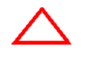
\includegraphics{images/1_triangle}
    \caption{Triangle drawn with Turtle Graphics \label{fig:triangle}}
    \end{center}
\end{figure}

With $n=1$ the production is applied once, which means that all $F$ Symbols in $\omega$ will be expanded. As $n$ increases, so does the complexity of the result. \autoref{fig:triangle_detail} shows the increasing detailed results of this L-System for $1 \leq n \leq 4$

\begin{figure}[!htp]
  \begin{center}
    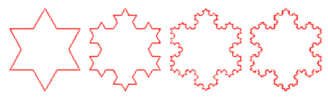
\includegraphics{images/2_triangle_detail}
    \caption{Expansion of the Triangle L-System \label{fig:triangle_detail}}
    \end{center}
\end{figure}

%%%%%%%%%%%%%%%%%%%%%%%%%%%%%%%%%%%%%%%%%%%%%%%%
%%%%%%%%%%%%%%%%%%%%%%%%%%%%%%%%%%%%%%%%%%%%%%%%
\section{Functionality}
\label{sec:functionality}

\subsection{Branching}
\label{subsec:branching}

Let's now add some more operator to the symbol list:

\begin{eqnarray}
    [ & \rightarrow &  push_state()  \nonumber \\
    ] & \rightarrow &  pop_state()   \nonumber
\end{eqnarray}

Where push\_state() is a function instruct the turtle system to store it's current state in a stack, and pop\_state() instructs it to reload the last saved state, removing it from the stack. With the introduction of a stack, the turtle can effectively recover previous states, allowing for branched geometries to be rendered, continued from a previous point of the geometry that is not the most recently drawn. For instance, consider now the following L-System and its corresponding result for different $n$ values:

\begin{eqnarray}
  \alpha  &=& 30                        \nonumber \\
  V       &=& \{F, -, +, [,\; ]\}       \nonumber \\
  \omega  &=& F                          \nonumber \\
  P       &=& \{F \rightarrow F[-F]F[+F]F\} \nonumber
%  \label{eq:example2}
\end{eqnarray}

\begin{figure}[!htp]
  \begin{center}
    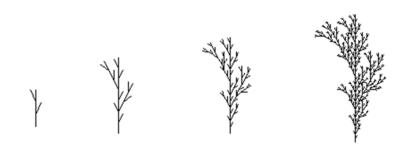
\includegraphics[width=\columnwidth]{images/3_tree}
    \caption{Trees drawn with Turtle Graphics \label{fig:tree}}
    \end{center}
\end{figure}

The stack operator can be useful to allow the turtle to explicity recover previous states, allowing complex geomtries that resemble weeds and other types of vegetation.

\subsection{Parametric L-Systems}
\label{subsec:parametric}

An L-System can support parameters which can be useful to use the same system to generate geometries with a certain degree of variety. For example, a generator for a tree leaf can be parameterized with the leaf's color and length, resulting in the creation of several different leafs which, even though are sharing a common structure, have some noticeable differentes between them.

Another useful capability of parameters is to allow the same productions to be used to achieve different results, according to the parameters that are give to them. The preivous example to render weeds can be extended with parameters to add some variety to the result.

A parametric L-System can also include conditional productions, so that they are only applied when their parameters meet a condition, as shown in the following example:

\begin{eqnarray}
  V       &=& \{F\}                                               \nonumber \\
  \omega  &=& F(4,4)                                              \nonumber \\
  P       &=& \{                                                  \nonumber \\
          & & F(x,y) : x \leq 3 \rightarrow F(x \times 2, x + y,  \nonumber \\
          & & \, F(x,y) : x >    3 \rightarrow F(x / y, 0\        \nonumber \\
          & & \}                                                  \nonumber
%  \label{eq:example3}
\end{eqnarray}

\subsection{Stochastic L-Systems}
\label{subsec:stochastic}

An L-System can also be parameterized with probabilistical values, allowing for a somewhat random effect to be added, creating more diverse and natural results. This is called a Stochastic L-System. Consider the following example:

\begin{eqnarray}
  V       &=& \{F, -, +\}                   \nonumber \\
  \omega  &=& F                             \nonumber \\
  P       &=& \{                            \nonumber \\
          & & F : (0.5) \rightarrow [+FF]F, \nonumber \\
          & & F : (0.5) \rightarrow [-FF]F, \nonumber \\
          & & \}                            \nonumber \\
%  \label{eq:example4}
\end{eqnarray}

In this system, when expanding the $F$ symbol, both productions might be used. However, unlike in the example shown in \autoref{subsec:parametric}, where the choice was determined by the parameters given to the system, here, the choice is probabilistical. There is a $50\%$ change for each production to be used each time. In this example, one production creates a branch on the right side of the structure, while the other does the same on the left side. So at each step, a branch will be created on a randomly choosen side. \autoref{fig:stochastic} shows four different results achieved using this L-System.

\begin{figure}[!htp]
  \begin{center}
    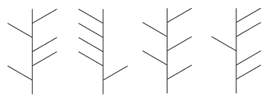
\includegraphics[width=0.6\columnwidth]{images/4_stochastic}
    \caption{Stochastic L-System structures \label{fig:stochastic}}
    \end{center}
\end{figure}



% turtle + l systems -> fractais

%end sec{example}

%%%%%%%%%%%%%%%%%%%%%%%%%%%%%%%%%%%%%%%%%%%%%%%%
%%%%%%%%%%%%%%%%%%%%%%%%%%%%%%%%%%%%%%%%%%%%%%%%
\section{Fractals}
\label{sec:fractals}

%%%%%%%%%%%%%%%%%%%%%%%%%%%%%%%%%%%%%%%%%%%%%%%%
%%%%%%%%%%%%%%%%%%%%%%%%%%%%%%%%%%%%%%%%%%%%%%%%
\section{Applications}
\label{sec:applications}


%%%%%%%%%%%%%%%%%%%%%%%%%%%%%%%%%%%%%%%%%%%%%%%%
%%%%%%%%%%%%%%%%%%%%%%%%%%%%%%%%%%%%%%%%%%%%%%%%
\section{L-Systems and Programming Languages}
\label{sec:languages}


\bibliographystyle{acmtog}
\nocite{*}
\bibliography{l_systems}


%\received{September 2z008}{March 2009}

\end{document}
